\section{Обзор предметной области}

\subsection{Существующие решения}

В данном разделе будут описаны существующие инструменты статического анализа, их возможности, преимущества и недостатки.

\subsubsection{SpotBugs}

Популярный анализатор исходного кода для языка Java. Распространяется в виде плагина для IntelliJ IDEA, задач для систем сборки Ant, Gradle и Maven, а также интерфейса командной строки. Внутри него реализованы различные эвристики, основанные на синтаксическом анализе текста программы. Хорошо справляется с поиском простых ошибок или опечаток, а также плохих практик в написании кода.

Возможности инструмента существенно расширяются при установке дополнения FindSecurityBugs \cite{fsbugs}, которое реализует некоторые алгоритмы для поиска уязвимостей, в том числе и taint-анализ. Вместе с этим модулем SpotBugs может находить ошибки в безопасности, например использование непроверенного пользовательского ввода в критических секциях программы (HTTP-запросы, работа с файловой системой и так далее).

Основным недостатком данного продукта является большое количество ложных срабатываний (от 40 до 60 процентов \cite{fsbugs-fp}), которые возникают из-за применения методов, основанных на исследовании исходного текста программы.

\subsubsection{Coverity}

Пакет программного обеспечения, состоящий из статического и динамического анализаторов кода на C++, Java, C\#, Scala и некоторых других языках. Внутри Coverity реализовано несколько подходов к поиску ошибок, в том числе и taint-анализ, который, прежде всего, используется для нахождения случаев нарушения безопасности, таких как SQL-инъекции или XSS (<<межсайтовый скриптинг>>).

Продукт активно используют для автоматической проверки критически важного кода, например, лаборатория реактивного движения НАСА тестировала с помощью него исходные коды марсохода Curiosity \cite{curiosity}.

Как и у многих рассматриваемых инструментов, существенный недостаток Coverity "--- частые ложноположительные срабатывания. 
В разных публикациях на тему измерения доли ошибочных предупреждений Coverity приводятся разные данные, но в среднем получается от 10 до 35 процентов \cite{coverity-fp-1, coverity-fp-2, coverity-fp-3}.

\subsubsection{CodeQL}

Инструмент статического анализа с открытым исходным кодом, а также поставляемый вместе с ним язык запросов, похожий на SQL, позволяющий проверять некоторые гипотезы относительно кода или идущих через него данных. Например, можно составить запросы на этом декларативном языке, которые проверят есть ли путь в графе потока данных от места пользовательского ввода до небезопасного участка кода, где эти данные применяются. Таким образом удаётся обнаружить такие уязвимости, как SQL-инъекция, XSS, разыменование нулевого указателя и некоторые другие.

Простейший сценарий использования состоит в том, чтобы просто запустить сканер с набором стандартных, написанных создателями, запросов, а затем просматривать результаты, среди которых в основном будут проблемы с качеством кода и проблемы с безопасностью. Однако более продуктивный сценарий включает в себя написание собственных запросов, исходя из специфики конкретного приложения. В этом заключается одновременно и основное преимущество, и главный недостаток данного продукта. С одной стороны пользователю предоставляется большая гибкость в написании запросов под собственные нужды. С другой стороны, чтобы начать эффективно пользоваться инструментом, нужно не просто придумать и написать релевантные для конкретного проекта запросы, а ещё и выучить непростой декларативный язык вместе со всем его спектром возможностей.

Корректно оценить частоту ложноположительных срабатываний может быть сложно, ведь результат напрямую зависит от набора пользовательских запросов, с которыми запускается CodeQL. Тем не менее существуют исследования, где проводятся подобные сравнения, например, в статье \cite{codeql-fp} указана доля ошибочных сообщений в 50 процентов, что довольно много.

\subsubsection{Infer}

Статический анализатор программ для Java, C и Objective-C, который способен отслеживать проблемы, вызванные разыменованиями нулевого указателя, утечками ресурсов и памяти, гонками данных в многопоточной среде и некоторыми другими ошибками.

Infer основан на сепарационной логике \cite{seplog} и технике bi-abduction \cite{biab}, что позволяет ему рассуждать о мутациях в памяти компьютера и выполнять глубокий анализ кода на предмет некорректного обращения с памятью. Отметим, что использование формальных подходов способствует меньшему количеству выдаваемых ложноположительных результатов по сравнению с описанными выше инструментами, а именно около 2 процентов \cite{infer-fp}. 
Тем не менее алгоритмы, реализованные внутри Infer, не обладают таким свойством, как теоретически полное отсутствие ложноположительных срабатываний. Другими словами, при любой реализации они будут, в отличие от, например, символьного исполнения, у которого такое свойство есть.

\subsubsection{Выводы}

Проведённый обзор существующих инструментов статического анализа показал, что многие популярные продукты, во-первых, допускают большое количество ложноположительных срабатываний, а во-вторых, проводят лишь поверхностный анализ, не обнаруживая редкие сценарии исполнения, приводящие к некорректному поведению программы. Одним из способов решения обозначенных недостатков является использование формальных методов математической логики. В данной работе предлагается применить технику символьного исполнения.

\newpage

\subsection{Символьное исполнение}

Символьное исполнение \cite{sym-3d, sym-sur} "--- это широко распространенная техника анализа программного обеспечения, которая позволяет для каждого из возможных путей исполнения найти соответствующий ему набор входных данных. В частности, метод способен обнаружить пути, ведущие к неожиданному результату работы программы, например, к выбрасыванию исключения.

\subsubsection{Описание алгоритма}\label{sec-sym-exec}

Символьное исполнение работает в условиях неопределенности входных данных. Неопределённые данные, другими словами \textit{символы} или \textit{символьные} переменные, являются абстракцией конкретных объектов или переменных, которыми оперирует код во время обычного исполнения. Символы, в отличие от конкретных переменных, могут принимать сразу целое множество значений, которые допускает соответствующий им тип данных. Эти абстракции хранятся в специальной \textit{символьной} памяти, состояние которой поддерживает алгоритм символьного исполнения в процессе своей работы. Помимо символьной памяти \var{memory}, в поддерживаемое состояние входят следующие данные:

\begin{itemize}
    \item текущая инструкция программы \var{stmt}, которую обрабатывает алгоритм.
    \item условие пути \var{pathCondition} в виде логической формулы, выражающее ограничения на символьные переменные для текущего пути исполнения.
    \item путь исполнения \var{path}, по которому мы пришли в это состояние.
\end{itemize}

В общих чертах опишем алгоритм символьного исполнения.

Изначально есть одно состояние, которое соответствует состоянию программы при её запуске.

Далее, если алгоритм встречает инструкцию без ветвления, то он просто обновляет текущее состояние с учётом полученной информации. Например, инструкция присваивания \var{x := 1} вызовет обновление ячейки символьной памяти, которая соответствует переменной \var{x}. 

Если же алгоритм встречает инструкцию с ветвлением, например, \var{if (\xi)}, то он дублирует текущее состояние \var{state}, получая два новых состояния \var{state_{if}} и \var{state_{else}}. В состоянии \var{state_{if}} обновляется условие пути так, будто бы $\xi$ выполняется, а в состоянии \var{state_{else}} условие пути обновляется так, будто бы $\xi$ не выполняется. Таким образом, получаются два состояния, соответствующие разветвлению. После чего оба условия проверяются на выполнимость, и, в случае невыполнимости какого-то из полученных условий, соответствующее состояние удаляется из рассмотрения.

Работа алгоритма продолжается до тех пор, пока состояние не придёт в конечную инструкцию или исполнение не завершится в результате нахождения ошибки в программе.

После завершения исполнения символьная память и условие пути конечного состояния \var{state_f} определяют ограничения на входные данные программы. Для того чтобы найти конкретные входные данные, которые удовлетворяют составленным ограничениям, используется SMT-решатель \cite{smt}. В итоге программа, запущенная на найденных входных данных, пройдёт тот же путь исполнения, что и конечное состояние \var{state_f}, из которого они были получены.

\subsubsection{Пример работы}

Для лучшего понимания концепции, рассмотрим пример работы символьной виртуальной машины на функции \var{example}.

\begin{code}
int example(int x, int y) {
    int a = 1;

    if (x > 27) {
        a += y;
    } else {
        a += 12;
    }

    return y / a;
}
\end{code}

\begin{figure}[ht]
    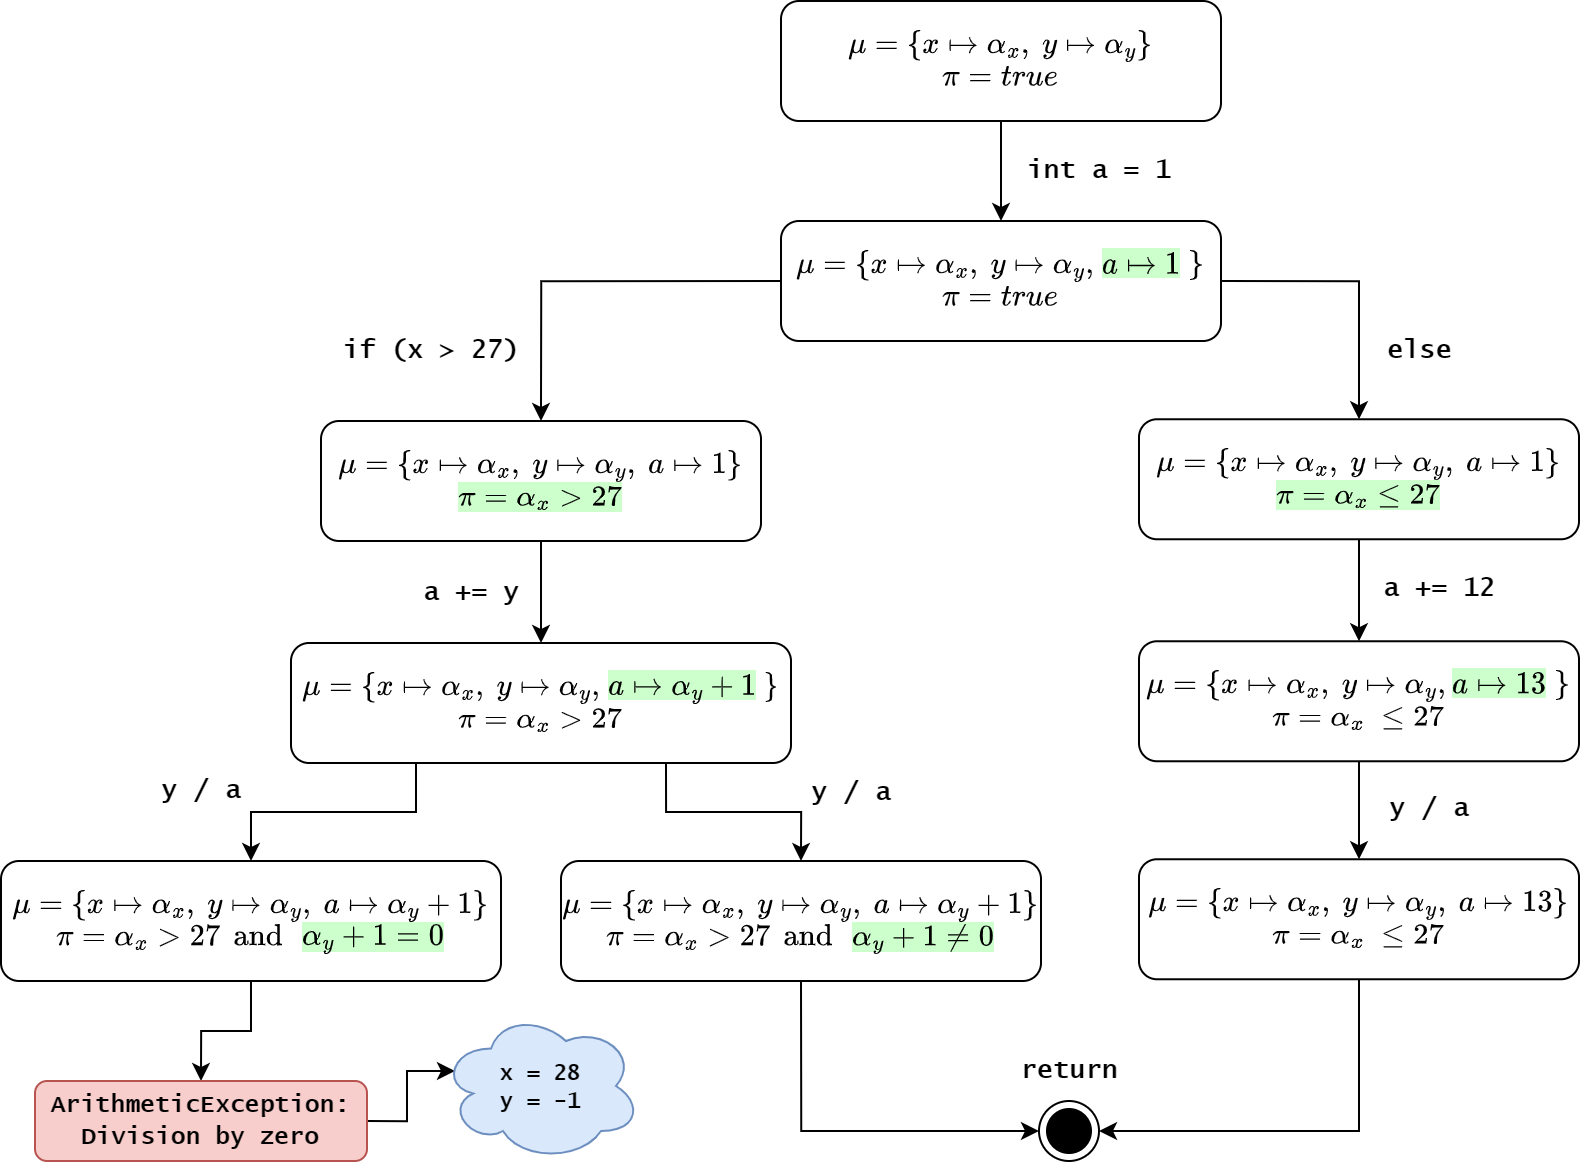
\includegraphics[scale=0.28]{images/se-example-200.png}
    \caption{\label{se-example} Схема символьного исполнения функции \var{example}.}
\end{figure}

По итогам анализа мы хотим ответить на вопрос, существуют ли какие-нибудь конкретные входные аргументы функции \var{example}, при которых в строке 10 выбрасывается исключение \verb|ArithmeticException: / by zero|, и, если существуют, то хотим найти их.

В схеме, представленной на рис. \ref{se-example}, прямоугольник "--- это одно состояние символьной машины. Оно хранит в себе символьную память и условие пути, которые для краткости обозначены $\mu$ и $\pi$ соответственно. Память $\mu$ в данном примере хранит для каждой переменной её символьное значение, то есть для $x$ это $\alpha_x$, а для $y$ "--- $\alpha_y$. Условие пути $\pi$ "--- это логическая формула со значениями символьных переменных, выполняемая на текущем пути исполнения. Переход от состояния к состоянию происходит при обработке некоторой инструкции исходного кода, записанной на соответствующем ребре графа состояний.

Изначально в $\mu$ лежат символьные переменные, на которые ещё не наложено ни одно ограничение, а $\pi$ "--- это всегда выполняющаяся формула, то есть просто $true$.

Обрабатывая инструкции исходного кода, символьная виртуальная машина поддерживает значения $\mu$ и $\pi$ в актуальном состоянии. Например, после строки \verb|int a = 1|, в $\mu$ запомнилась переменная $a$ и её значение $1$. А после обработки условного оператора \verb|if (x > 27)|, исполнение разветвилось на два пути, в каждом из которых обновилось $\pi$: в ветке \verb|if| оно равно $\alpha_x > 27$, а в ветке \verb|else| равно $\alpha_x \le 27$.

В некоторый момент алгоритм обнаруживает состояние, которое ведёт к выбрасыванию исключения. После этого он обращается к SMT-решателю с запросом найти конкретные значения $\alpha_x$ и $\alpha_y$, которые выполняют формулу $\pi = \alpha_x > 27 \land \alpha_y + 1 = 0$, или же сообщить, что решений не существует. В данном примере формула оказывается выполнима, и SMT-решатель возвращает набор $\alpha_x = 28, ~\alpha_y = -1$. Таким образом, удалось автоматически сгенерировать тестовый случай \verb|example(28, -1)|, который приводит к падению программы из-за необработанного исключения.

\newpage

\subsection{UnitTestBot}

UnitTestBot "--- инструмент, который по исходному коду на языке Java автоматически генерирует модульные тесты, пытаясь при этом максимизировать количество покрытых инструкций. UnitTestBot использует для работы собственную символьную виртуальную машину, что даёт возможность ожидать от сгенерированных тестов теоретически полного покрытия кода.

Продукт поставляется как плагин для среды разработки IntelliJ IDEA, что позволяет запускать генерацию тестов, используя удобный пользовательский интерфейс. Инструмент поддерживает популярные системы сборки Gradle и Maven, поэтому его достаточно легко применить на любом проекте, написанном на языке Java. Помимо всего прочего, UnitTestBot предоставляет пользователям множество конфигурируемых параметров своей работы, гибко настраиваясь под нужды тестирования конкретного проекта. В частности, программист может задать количество времени в секундах, которое будет доступно инструменту для генерации тестов.

\subsubsection{Архитектура}\label{sec-utbot-arch}

В данном подразделе будет проведён обзор общей архитектуры проекта, а также некоторых деталей реализации символьной виртуальной машины, которую использует UnitTestBot.

На рис. \ref{utbot-arch} представлена высокоуровневая диаграмма ключевых модулей проекта. 
%Некоторые модули, в особенности те, которые не будут каким-либо образом задействованы или модифицированы в данной работе, не отражены на данной схеме для краткости.
Рассмотрим каждую компоненту подробнее.

\begin{figure}[ht]
    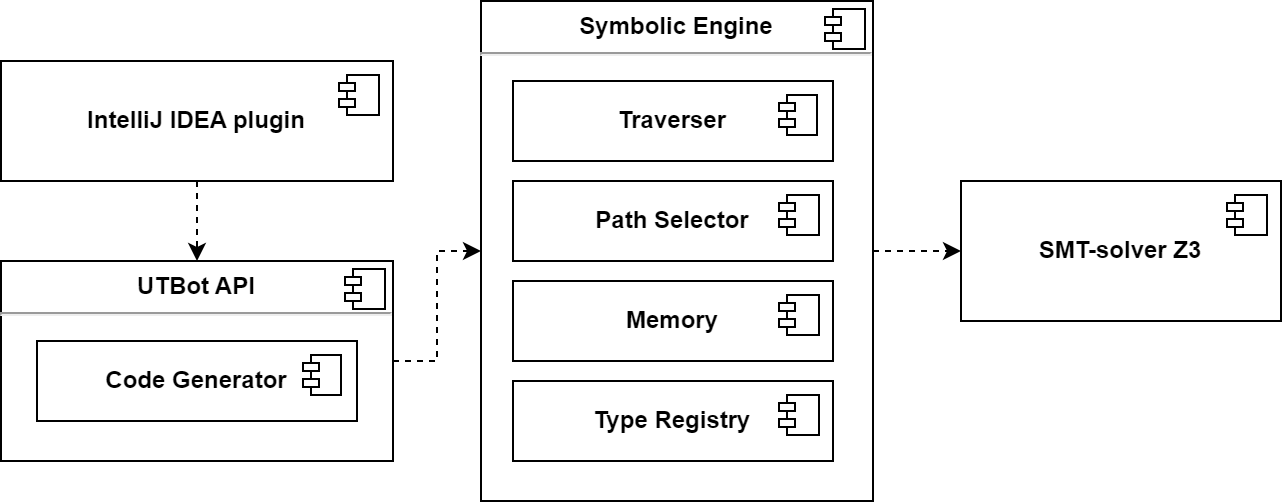
\includegraphics[scale=0.35]{images/utbot-arch-200.png}
    \caption{\label{utbot-arch} Диаграмма основных модулей проекта UnitTestBot.}
\end{figure}

Плагин для IntelliJ IDEA задаёт представление интерфейса в указанной среде разработки. Модуль собирает с пользовательского проекта все нужные для генерации тестов данные, например структуру классов или файлы с Java байт-кодом. Другими словами, является точкой входа в приложение, позволяя настраивать и запускать генерацию тестов.

Пакет \verb|UTBot API| отвечает за формирование входных данных для генерации тестов, запуск символьной виртуальной машины и возвращение результата её работы в удобном для вызывающего кода виде. Типичный сценарий использования данного модуля выглядит следующим образом. Плагин для IntelliJ IDEA совершает запрос на генерацию тестов, передавая байт-код пользовательских классов и все остальные необходимые данные. После чего описываемый компонент преобразует пришедшие данные в нужный формат и запускает на них символьное исполнение. Результат работы символьной машины поступает в \verb|Code Generator|, который генерирует код тестов на языке Java, соответствующий найденным тестовым случаям. В итоге полученный файл с тестами возвращается в модуль плагина и отображается на экране пользователя.

Модуль \verb|Symbolic Engine| "--- это символьная виртуальная машина внутри UnitTestBot, центральный и самый сложный компонент проекта. В качестве входных данных, он ожидает байт-код одного метода\footnote{На самом деле символьная машина работает не с обычным Java байт-кодом, а с упрощённым трёхадресным кодом. Однако для простоты, эта деталь реализации опускается.}, а результатом исполнения является множество тестовых случаев, то есть наборов входных параметров метода. В процессе своей работы модуль делает запросы к SMT-решателю Z3 \cite{z3}, как было описано в общем алгоритме символьного исполнения (в разделе \ref{sec-sym-exec}).

Работа модуля высокоуровнево выглядит следующим образом. На каждом шаге текущее состояние извлекается из \verb|Path Selector|, затем обрабатывается в \verb|Traverser|, который возвращает несколько новых состояний. Для каждого из полученных состояний проверяется, является ли оно терминальным. Если да, то оно запоминается как результат исполнения, а иначе кладётся в очередь состояний внутри \verb|Path Selector|. 

Теперь рассмотрим обязанности наиболее важных классов данного модуля подробнее.

\begin{itemize}
    \item \verb|Path Selector| "--- это класс, принимающий решение о том, какая инструкция программы должна быть обработана следующей. Хранит внутри себя некоторый список доступных состояний (при старте только одно начальное), позволяет добавлять туда новое состояние, а также извлекать некоторое следующее. Какое именно состояние будет извлечено из списка, определяется на основании реализованной внутри эвристики.
    \item \verb|Traverser| обрабатывает поданное на вход состояние. Он содержит информацию о графе потока управления, иерархии классов в программе и системе символьных типов. \verb|Traverser|, в зависимости от состояния и текущей инструкции, создаёт набор новых состояний, в которых обновлена символьная память и добавлены необходимые логические ограничения для соответствующего пути исполнения. Описанное множество состояний и является результатом работы класса.
    \item \verb|Memory| отвечает за символьное представление памяти состояния в программе. Высокоуровнево работает ровно так, как было описано в главе про символьное исполнение (\ref{sec-sym-exec}).
    \item \verb|Type Registry| "--- важный компонент, который содержит информацию о системе типов в анализируемом коде. Даёт возможность узнать тип символьного объекта во время исполнения.
\end{itemize}

\subsubsection{Пример работы}

Рассмотрим пример работы инструмента UnitTestBot на уже знакомой функции \var{example}, которая теперь является методом класса \var{Main}.

\begin{code}
public class Main {

    int example(int x, int y) {
        int a = 1;

        if (x > 27) {
            a += y;
        } else {
            a += 12;
        }

        return y / a;
    }
}
\end{code}

Программист запускает генерацию тестов, используя интерфейс плагина для IntelliJ IDEA, при этом указав количество отведённого на генерацию тестов времени 10 секунд.

Конфигурация, Java байт-код, структура классов, а также вся остальная необходимая информация преобразуется в модуле \verb|UTBot API| и передается в \verb|Symbolic Engine| в ожидаемом для него виде. Тот, в свою очередь, с помощью символьного исполнения находит 2 набора входных параметров функции.
\begin{enumerate}
    \item Набор $x = 27, ~ y = -255$ покрывает все строчки, кроме седьмой, и возвращает $-19$ в качестве результата метода \var{example}.
    \item Набор $x = 28, ~ y = -1$ покрывает оставшуюся непокрытой строку номер 7, а также инициирует выброс необработанного исключения \verb|ArithmeticException: / by zero| в строке 12.
\end{enumerate}

Результат работы \verb|Symbolic Engine| передаётся в \verb|Code Generator|, который для данного примера генерирует следующий код.

\begin{code}
import org.junit.jupiter.api.Test;

import static org.junit.jupiter.api.Assertions.assertEquals;

public final class MainTest {

    @Test
    public void testExample1() {
        Main main = new Main();
        int actual = main.example(27, -255);
        assertEquals(-19, actual);
    }

    @Test
    public void testExample2() {
        Main main = new Main();
        main.example(28, -1);
    }
}
\end{code}

Если запустить полученные тесты, то второй завершится с ошибкой. Это является ожидаемым поведением инструмента, ведь программист забыл обработать возможное исключение. Об этом ему сообщается в виде теста, который не проходит.

\newpage

\subsection{Taint-анализ}

Taint-анализ \cite{taint} "--- это технология, позволяющая отслеживать распространение непроверенных внешних данных по программе. Попадание таких данных в критические секции кода может привести к различным уязвимостям, включая SQL-инъекцию, межсайтовый скриптинг (XSS) и многие другие. Злоумышленники могут использовать эти уязвимости для нарушения корректной работы системы, получения конфиденциальных данных или проведения других несанкционированных операций. Taint-анализ помогает находить описанные ошибки ещё на этапе компиляции. Отметим, что методика может быть применена и во время непосредственного выполнения программы \cite{dyn-taint}, однако данная работа не будет затрагивать эту область.

\subsubsection{Описание алгоритма}

Ключевая идея подхода заключается в том, что любая переменная, которая может быть изменена внешним пользователем, представляет потенциальную угрозу безопасности. Если эта переменная используется в некотором выражении, то значение этого выражения также становится подозрительным. Далее, алгоритм отслеживает и оповещает о ситуациях, когда какая-либо из этих \textit{помеченных} переменных используется для выполнения опасных команд, например, прямых запросов в базу данных или в операционную систему компьютера.

Для своей работы, taint-анализ требует конфигурацию, в которой методам программы можно назначить одну из следующих ролей.

\begin{itemize}
    \item \verb|Taint source| "--- \textit{источник} непроверенных данных. К примеру, это может быть метод считывания пользовательского ввода или же метод получения параметра пришедшего HTTP-запроса. Переменные, в которые записывается результат выполнения \verb|Taint source|, называются \textit{помеченными}. Семантика метода определяет, какая именно метка будет наложена на переменную. Причём имя метки может быть совершенно произвольным, так как его выбирает тот, кто пишет конфигурацию. \\
    Например, может быть задано, что функция \verb|getPassword()| накладывает метку \verb|"sensitive-data"| на своё возвращаемое значение.
    \item \verb|Taint sink| "--- \textit{приёмник}, некоторая критическая секция приложения. Это может быть метод прямого обращения к базе данных или файловой системе, а также любая другая потенциально опасная операция. Для \verb|Taint sink| можно задать набор меток, переменные с которыми не должны в него просочиться. \\
    К примеру, если значение с меткой \verb|"sensitive-data"| передаётся в функцию журналирования, которая печатает свои аргументы напрямую в консоль, то это ошибка разработчика, так как происходит утечка данных.
\end{itemize}

Помимо источников и приёмников, есть ещё две вспомогательные сущности, которые нужны для расширения возможностей алгоритма.
\begin{itemize}
    \item \verb|Taint pass| "--- это функция, которая помечает возвращаемое значение с учётом меток в её аргументах. В зависимости от реализации, метки могут накладываться не только на результат метода, но и на объект \verb|this|, и на входные параметры. \\
    Например, в конфигурации может быть установлено, что метод конкатенации строк \verb|concat(String a, String b)| помечает свой результат всеми метками из \var{a} и из \var{b}.
    \item \verb|Taint cleaner| "--- это функция, которая удаляет заданный набор меток из переданных аргументов. Чаще всего, это некоторый метод валидации, который проверяет, что пользователь ввёл данные в ожидаемом формате. \\
    К примеру, метод \verb|validateEmail(String email)| удаляет метку \verb|XSS| при успешном прохождении проверок, так как теперь в строке \var{email} точно нет непроверенных данных, которые могут привести к уязвимости межсайтового скриптинга.
\end{itemize}

Алгоритм taint-анализа сканирует граф потока данных, пытаясь обнаружить маршрут между методом из множества \verb|Taint sources| и методом из \verb|Taint sinks|. Основной проблемой классического алгоритма, как и у всех методов неточного анализа, является большое количество ложноположительных срабатываний. Однако существуют научные публикации \cite{sym-taint}, в которых данная проблема решается с помощью применения символьного исполнения. Другими словами, если встроить taint-анализ непосредственно внутрь символьной виртуальной машины, то удаётся практически полностью избавиться от ложных результатов, а также заодно получить конкретные входные данные, реализующие найденный путь от источника к приёмнику. Последний подход и будет реализован в данной работе.

\subsubsection{Пример работы}

Рассмотрим пример простой функции, в которой есть уязвимость вида SQL-инъекция: если злоумышленник введёт в переменную \var{name} строку \verb|"name'); DROP TABLE Employees; --"|, то у него получится удалить таблицу \verb|Employees| вместе со всеми данными, которые в ней хранились.

\begin{code}
void example(Connection connection) throws SQLException {
    Scanner sc = new Scanner(System.in);
    String name = sc.nextLine();

    Statement stmt = connection.createStatement();
    String query = 
        "INSERT INTO Employees(name) VALUES('"
        .concat(name)
        .concat("')");
    stmt.executeUpdate(query);
}
\end{code}

Для работы taint-анализа нужно сначала задать правильную конфигурацию.
\begin{itemize}
    \item \verb|Taint source| "--- метод \verb|nextLine| класса \verb|java.util.Scanner|, который добавляет к возвращаемому значению метку \verb|"user-input"|.
    \item \verb|Taint pass| "--- метод \verb|concat| класса \verb|java.lang.String|, который пропускает через себя метку \verb|"user-input"|, полученную либо у первого аргумента, либо у объекта, на котором этот метод вызывается (то есть у \verb|this|).
    \item \verb|Taint sink| "--- метод \verb|executeUpdate| класса \verb|java.sql.Statement|, который отслеживает переменные, помеченные \verb|"user-input"|.
\end{itemize}

Любая корректная реализация taint-анализа должна найти в этом коде ошибку: переменная \var{query} с меткой \verb|"user-input"| передаётся в приёмник \verb|executeUpdate|. 

Важно отметить, что в обязанности алгоритма не входит нахождение конкретных данных, которые бы смог ввести злоумышленник, чтобы навредить программе. Требуется лишь обнаружить маршрут, соединяющий источник и приёмник.
